\documentclass[1p]{elsarticle_modified}
%\bibliographystyle{elsarticle-num}

%\usepackage[colorlinks]{hyperref}
%\usepackage{abbrmath_seonhwa} %\Abb, \Ascr, \Acal ,\Abf, \Afrak
\usepackage{amsfonts}
\usepackage{amssymb}
\usepackage{amsmath}
\usepackage{amsthm}
\usepackage{scalefnt}
\usepackage{amsbsy}
\usepackage{kotex}
\usepackage{caption}
\usepackage{subfig}
\usepackage{color}
\usepackage{graphicx}
\usepackage{xcolor} %% white, black, red, green, blue, cyan, magenta, yellow
\usepackage{float}
\usepackage{setspace}
\usepackage{hyperref}

\usepackage{tikz}
\usetikzlibrary{arrows}

\usepackage{multirow}
\usepackage{array} % fixed length table
\usepackage{hhline}

%%%%%%%%%%%%%%%%%%%%%
\makeatletter
\renewcommand*\env@matrix[1][\arraystretch]{%
	\edef\arraystretch{#1}%
	\hskip -\arraycolsep
	\let\@ifnextchar\new@ifnextchar
	\array{*\c@MaxMatrixCols c}}
\makeatother %https://tex.stackexchange.com/questions/14071/how-can-i-increase-the-line-spacing-in-a-matrix
%%%%%%%%%%%%%%%

\usepackage[normalem]{ulem}

\newcommand{\msout}[1]{\ifmmode\text{\sout{\ensuremath{#1}}}\else\sout{#1}\fi}
%SOURCE: \msout is \stkout macro in https://tex.stackexchange.com/questions/20609/strikeout-in-math-mode

\newcommand{\cancel}[1]{
	\ifmmode
	{\color{red}\msout{#1}}
	\else
	{\color{red}\sout{#1}}
	\fi
}

\newcommand{\add}[1]{
	{\color{blue}\uwave{#1}}
}

\newcommand{\replace}[2]{
	\ifmmode
	{\color{red}\msout{#1}}{\color{blue}\uwave{#2}}
	\else
	{\color{red}\sout{#1}}{\color{blue}\uwave{#2}}
	\fi
}

\newcommand{\Sol}{\mathcal{S}} %segment
\newcommand{\D}{D} %diagram
\newcommand{\A}{\mathcal{A}} %arc


%%%%%%%%%%%%%%%%%%%%%%%%%%%%%5 test

\def\sl{\operatorname{\textup{SL}}(2,\Cbb)}
\def\psl{\operatorname{\textup{PSL}}(2,\Cbb)}
\def\quan{\mkern 1mu \triangleright \mkern 1mu}

\theoremstyle{definition}
\newtheorem{thm}{Theorem}[section]
\newtheorem{prop}[thm]{Proposition}
\newtheorem{lem}[thm]{Lemma}
\newtheorem{ques}[thm]{Question}
\newtheorem{cor}[thm]{Corollary}
\newtheorem{defn}[thm]{Definition}
\newtheorem{exam}[thm]{Example}
\newtheorem{rmk}[thm]{Remark}
\newtheorem{alg}[thm]{Algorithm}

\newcommand{\I}{\sqrt{-1}}
\begin{document}

%\begin{frontmatter}
%
%\title{Boundary parabolic representations of knots up to 8 crossings}
%
%%% Group authors per affiliation:
%\author{Yunhi Cho} 
%\address{Department of Mathematics, University of Seoul, Seoul, Korea}
%\ead{yhcho@uos.ac.kr}
%
%
%\author{Seonhwa Kim} %\fnref{s_kim}}
%\address{Center for Geometry and Physics, Institute for Basic Science, Pohang, 37673, Korea}
%\ead{ryeona17@ibs.re.kr}
%
%\author{Hyuk Kim}
%\address{Department of Mathematical Sciences, Seoul National University, Seoul 08826, Korea}
%\ead{hyukkim@snu.ac.kr}
%
%\author{Seokbeom Yoon}
%\address{Department of Mathematical Sciences, Seoul National University, Seoul, 08826,  Korea}
%\ead{sbyoon15@snu.ac.kr}
%
%\begin{abstract}
%We find all boundary parabolic representation of knots up to 8 crossings.
%
%\end{abstract}
%\begin{keyword}
%    \MSC[2010] 57M25 
%\end{keyword}
%
%\end{frontmatter}

%\linenumbers
%\tableofcontents
%
\newcommand\colored[1]{\textcolor{white}{\rule[-0.35ex]{0.8em}{1.4ex}}\kern-0.8em\color{red} #1}%
%\newcommand\colored[1]{\textcolor{white}{ #1}\kern-2.17ex	\textcolor{white}{ #1}\kern-1.81ex	\textcolor{white}{ #1}\kern-2.15ex\color{red}#1	}

{\Large $\underline{12n_{0425}~(K12n_{0425})}$}

\setlength{\tabcolsep}{10pt}
\renewcommand{\arraystretch}{1.6}
\vspace{1cm}\begin{tabular}{m{100pt}>{\centering\arraybackslash}m{274pt}}
\multirow{5}{120pt}{
	\centering
	\includegraphics[width=112pt]{../../../GIT/diagram.site/Diagrams/png/2514_12n_0425.png}\\
\ \ \ A knot diagram\footnotemark}&
\allowdisplaybreaks
\textbf{Linearized knot diagam} \\
\cline{2-2}
 &
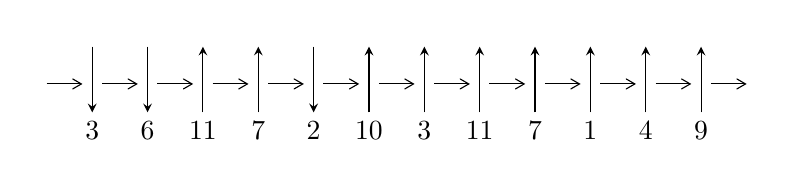
\begin{tikzpicture}[x=20pt, y=17pt]
	% nodes
	\node (C0) at (0, 0) {};
	\node (C1) at (1, 0) {};
	\node (C1U) at (1, +1) {};
	\node (C1D) at (1, -1) {3};

	\node (C2) at (2, 0) {};
	\node (C2U) at (2, +1) {};
	\node (C2D) at (2, -1) {6};

	\node (C3) at (3, 0) {};
	\node (C3U) at (3, +1) {};
	\node (C3D) at (3, -1) {11};

	\node (C4) at (4, 0) {};
	\node (C4U) at (4, +1) {};
	\node (C4D) at (4, -1) {7};

	\node (C5) at (5, 0) {};
	\node (C5U) at (5, +1) {};
	\node (C5D) at (5, -1) {2};

	\node (C6) at (6, 0) {};
	\node (C6U) at (6, +1) {};
	\node (C6D) at (6, -1) {10};

	\node (C7) at (7, 0) {};
	\node (C7U) at (7, +1) {};
	\node (C7D) at (7, -1) {3};

	\node (C8) at (8, 0) {};
	\node (C8U) at (8, +1) {};
	\node (C8D) at (8, -1) {11};

	\node (C9) at (9, 0) {};
	\node (C9U) at (9, +1) {};
	\node (C9D) at (9, -1) {7};

	\node (C10) at (10, 0) {};
	\node (C10U) at (10, +1) {};
	\node (C10D) at (10, -1) {1};

	\node (C11) at (11, 0) {};
	\node (C11U) at (11, +1) {};
	\node (C11D) at (11, -1) {4};

	\node (C12) at (12, 0) {};
	\node (C12U) at (12, +1) {};
	\node (C12D) at (12, -1) {9};
	\node (C13) at (13, 0) {};

	% arrows
	\draw[->,>={angle 60}]
	(C0) edge (C1) (C1) edge (C2) (C2) edge (C3) (C3) edge (C4) (C4) edge (C5) (C5) edge (C6) (C6) edge (C7) (C7) edge (C8) (C8) edge (C9) (C9) edge (C10) (C10) edge (C11) (C11) edge (C12) (C12) edge (C13) ;	\draw[->,>=stealth]
	(C1U) edge (C1D) (C2U) edge (C2D) (C3D) edge (C3U) (C4D) edge (C4U) (C5U) edge (C5D) (C6D) edge (C6U) (C7D) edge (C7U) (C8D) edge (C8U) (C9D) edge (C9U) (C10D) edge (C10U) (C11D) edge (C11U) (C12D) edge (C12U) ;
	\end{tikzpicture} \\
\hhline{~~} \\& 
\textbf{Solving Sequence} \\ \cline{2-2} 
 &
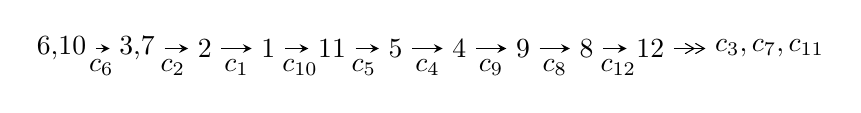
\begin{tikzpicture}[x=23pt, y=7pt]
	% node
	\node (A0) at (-1/8, 0) {6,10};
	\node (A1) at (17/16, 0) {3,7};
	\node (A2) at (17/8, 0) {2};
	\node (A3) at (25/8, 0) {1};
	\node (A4) at (33/8, 0) {11};
	\node (A5) at (41/8, 0) {5};
	\node (A6) at (49/8, 0) {4};
	\node (A7) at (57/8, 0) {9};
	\node (A8) at (65/8, 0) {8};
	\node (A9) at (73/8, 0) {12};
	\node (C1) at (1/2, -1) {$c_{6}$};
	\node (C2) at (13/8, -1) {$c_{2}$};
	\node (C3) at (21/8, -1) {$c_{1}$};
	\node (C4) at (29/8, -1) {$c_{10}$};
	\node (C5) at (37/8, -1) {$c_{5}$};
	\node (C6) at (45/8, -1) {$c_{4}$};
	\node (C7) at (53/8, -1) {$c_{9}$};
	\node (C8) at (61/8, -1) {$c_{8}$};
	\node (C9) at (69/8, -1) {$c_{12}$};
	\node (A10) at (11, 0) {$c_{3},c_{7},c_{11}$};

	% edge
	\draw[->,>=stealth]	
	(A0) edge (A1) (A1) edge (A2) (A2) edge (A3) (A3) edge (A4) (A4) edge (A5) (A5) edge (A6) (A6) edge (A7) (A7) edge (A8) (A8) edge (A9) ;
	\draw[->>,>={angle 60}]	
	(A9) edge (A10);
\end{tikzpicture} \\ 

\end{tabular} \\

\footnotetext{
The image of knot diagram is generated by the software ``\textbf{Draw programme}" developed by Andrew Bartholomew(\url{http://www.layer8.co.uk/maths/draw/index.htm\#Running-draw}), where we modified some parts for our purpose(\url{https://github.com/CATsTAILs/LinksPainter}).
}\phantom \\ \newline 
\centering \textbf{Ideals for irreducible components\footnotemark of $X_{\text{par}}$} 
 
\begin{align*}
I^u_{1}&=\langle 
-3141 u^{13}-16485 u^{12}+\cdots+48031 b-35243,\;-17396 u^{13}+34122 u^{12}+\cdots+48031 a-53374,\\
\phantom{I^u_{1}}&\phantom{= \langle  }u^{14}-2 u^{13}+2 u^{12}+2 u^{11}- u^{10}+5 u^9- u^8-3 u^7+16 u^6+14 u^5-7 u^4-4 u^3+5 u^2-1\rangle \\
I^u_{2}&=\langle 
u^7+u^6+2 u^5- u^3-3 u^2+b- u-1,\;u^6+u^5+2 u^4- u^2+a-2 u,\;u^8+2 u^7+3 u^6+u^5-2 u^4-5 u^3-3 u^2+1\rangle \\
I^u_{3}&=\langle 
-18446302691 u^{17}+75111115865 u^{16}+\cdots+37469236469 b+161494737225,\\
\phantom{I^u_{3}}&\phantom{= \langle  }1420585009695 u^{17}-6247662256333 u^{16}+\cdots+412161601159 a-27133691702098,\\
\phantom{I^u_{3}}&\phantom{= \langle  }u^{18}-5 u^{17}+\cdots-60 u+11\rangle \\
I^u_{4}&=\langle 
- u^6-3 u^5-6 u^4-7 u^3-5 u^2+b-2 u,\;u^6+3 u^5+7 u^4+10 u^3+11 u^2+a+8 u+3,\\
\phantom{I^u_{4}}&\phantom{= \langle  }u^8+4 u^7+10 u^6+16 u^5+18 u^4+14 u^3+7 u^2+2 u+1\rangle \\
\\
\end{align*}
\raggedright * 4 irreducible components of $\dim_{\mathbb{C}}=0$, with total 48 representations.\\
\footnotetext{All coefficients of polynomials are rational numbers. But the coefficients are sometimes approximated in decimal forms when there is not enough margin.}
\newpage
\renewcommand{\arraystretch}{1}
\centering \section*{I. $I^u_{1}= \langle -3141 u^{13}-16485 u^{12}+\cdots+48031 b-35243,\;-17396 u^{13}+34122 u^{12}+\cdots+48031 a-53374,\;u^{14}-2 u^{13}+\cdots+5 u^2-1 \rangle$}
\flushleft \textbf{(i) Arc colorings}\\
\begin{tabular}{m{7pt} m{180pt} m{7pt} m{180pt} }
\flushright $a_{6}=$&$\begin{pmatrix}1\\0\end{pmatrix}$ \\
\flushright $a_{10}=$&$\begin{pmatrix}0\\u\end{pmatrix}$ \\
\flushright $a_{3}=$&$\begin{pmatrix}0.362183 u^{13}-0.710416 u^{12}+\cdots-0.735608 u+1.11124\\0.0653953 u^{13}+0.343216 u^{12}+\cdots+0.546876 u+0.733755\end{pmatrix}$ \\
\flushright $a_{7}=$&$\begin{pmatrix}1\\- u^2\end{pmatrix}$ \\
\flushright $a_{2}=$&$\begin{pmatrix}0.427578 u^{13}-0.367200 u^{12}+\cdots-0.188732 u+1.84500\\0.0653953 u^{13}+0.343216 u^{12}+\cdots+0.546876 u+0.733755\end{pmatrix}$ \\
\flushright $a_{1}=$&$\begin{pmatrix}1\\-1.57877 u^{13}+2.67779 u^{12}+\cdots-6.70952 u-2.45421\end{pmatrix}$ \\
\flushright $a_{11}=$&$\begin{pmatrix}u\\-0.479753 u^{13}+0.602444 u^{12}+\cdots-1.45421 u-1.57877\end{pmatrix}$ \\
\flushright $a_{5}=$&$\begin{pmatrix}-0.747705 u^{13}+1.28783 u^{12}+\cdots-4.39699 u-0.909059\\-1.10989 u^{13}+1.99825 u^{12}+\cdots-3.66139 u-2.02030\end{pmatrix}$ \\
\flushright $a_{4}=$&$\begin{pmatrix}0.552518 u^{13}-0.954071 u^{12}+\cdots+0.0120964 u+1.31881\\-1.43745 u^{13}+2.65352 u^{12}+\cdots-4.96161 u-2.37884\end{pmatrix}$ \\
\flushright $a_{9}=$&$\begin{pmatrix}- u\\u^3+u\end{pmatrix}$ \\
\flushright $a_{8}=$&$\begin{pmatrix}0.266224 u^{13}-0.584622 u^{12}+\cdots-0.520247 u+0.357061\\-0.967708 u^{13}+1.43022 u^{12}+\cdots-3.29920 u-2.00635\end{pmatrix}$ \\
\flushright $a_{12}=$&$\begin{pmatrix}0.357061 u^{13}-0.447898 u^{12}+\cdots+1.57877 u+1.47975\\-1.88366 u^{13}+2.89045 u^{12}+\cdots-8.64535 u-3.20018\end{pmatrix}$\\&\end{tabular}
\flushleft \textbf{(ii) Obstruction class $= -1$}\\~\\
\flushleft \textbf{(iii) Cusp Shapes $= \frac{368903}{48031} u^{13}-\frac{551900}{48031} u^{12}+\cdots+\frac{897392}{48031} u+\frac{1052546}{48031}$}\\~\\
\newpage\renewcommand{\arraystretch}{1}
\flushleft \textbf{(iv) u-Polynomials at the component}\newline \\
\begin{tabular}{m{50pt}|m{274pt}}
Crossings & \hspace{64pt}u-Polynomials at each crossing \\
\hline $$\begin{aligned}c_{1}\end{aligned}$$&$\begin{aligned}
&u^{14}+7 u^{13}+\cdots+128 u+4
\end{aligned}$\\
\hline $$\begin{aligned}c_{2},c_{5}\end{aligned}$$&$\begin{aligned}
&u^{14}+5 u^{13}+\cdots-4 u+2
\end{aligned}$\\
\hline $$\begin{aligned}c_{3},c_{7},c_{11}\end{aligned}$$&$\begin{aligned}
&u^{14}-2 u^{13}+\cdots+3 u+1
\end{aligned}$\\
\hline $$\begin{aligned}c_{4}\end{aligned}$$&$\begin{aligned}
&u^{14}+7 u^{13}+\cdots-27 u-1
\end{aligned}$\\
\hline $$\begin{aligned}c_{6},c_{9},c_{10}\end{aligned}$$&$\begin{aligned}
&u^{14}+2 u^{13}+\cdots+5 u^2-1
\end{aligned}$\\
\hline $$\begin{aligned}c_{8}\end{aligned}$$&$\begin{aligned}
&u^{14}+11 u^{13}+\cdots-48 u-32
\end{aligned}$\\
\hline $$\begin{aligned}c_{12}\end{aligned}$$&$\begin{aligned}
&u^{14}-11 u^{13}+\cdots+112 u+26
\end{aligned}$\\
\hline
\end{tabular}\\~\\
\newpage\renewcommand{\arraystretch}{1}
\flushleft \textbf{(v) Riley Polynomials at the component}\newline \\
\begin{tabular}{m{50pt}|m{274pt}}
Crossings & \hspace{64pt}Riley Polynomials at each crossing \\
\hline $$\begin{aligned}c_{1}\end{aligned}$$&$\begin{aligned}
&y^{14}-7 y^{13}+\cdots-11904 y+16
\end{aligned}$\\
\hline $$\begin{aligned}c_{2},c_{5}\end{aligned}$$&$\begin{aligned}
&y^{14}-7 y^{13}+\cdots-128 y+4
\end{aligned}$\\
\hline $$\begin{aligned}c_{3},c_{7},c_{11}\end{aligned}$$&$\begin{aligned}
&y^{14}-22 y^{13}+\cdots-17 y+1
\end{aligned}$\\
\hline $$\begin{aligned}c_{4}\end{aligned}$$&$\begin{aligned}
&y^{14}-69 y^{13}+\cdots-481 y+1
\end{aligned}$\\
\hline $$\begin{aligned}c_{6},c_{9},c_{10}\end{aligned}$$&$\begin{aligned}
&y^{14}+10 y^{12}+\cdots-10 y+1
\end{aligned}$\\
\hline $$\begin{aligned}c_{8}\end{aligned}$$&$\begin{aligned}
&y^{14}-35 y^{13}+\cdots+2304 y+1024
\end{aligned}$\\
\hline $$\begin{aligned}c_{12}\end{aligned}$$&$\begin{aligned}
&y^{14}-47 y^{13}+\cdots-20136 y+676
\end{aligned}$\\
\hline
\end{tabular}\\~\\
\newpage\flushleft \textbf{(vi) Complex Volumes and Cusp Shapes}
$$\begin{array}{c|c|c}  
\text{Solutions to }I^u_{1}& \I (\text{vol} + \sqrt{-1}CS) & \text{Cusp shape}\\
 \hline 
\begin{aligned}
u &= -0.955042 + 0.173183 I \\
a &= \phantom{-}0.56818 + 1.84710 I \\
b &= -0.847861 - 0.494590 I\end{aligned}
 & \phantom{-}1.67693 - 2.03514 I & \phantom{-}12.04529 + 3.68045 I \\ \hline\begin{aligned}
u &= -0.955042 - 0.173183 I \\
a &= \phantom{-}0.56818 - 1.84710 I \\
b &= -0.847861 + 0.494590 I\end{aligned}
 & \phantom{-}1.67693 + 2.03514 I & \phantom{-}12.04529 - 3.68045 I \\ \hline\begin{aligned}
u &= -0.776212 + 0.543476 I \\
a &= \phantom{-}0.165614 + 0.941776 I \\
b &= -0.818876 - 1.029970 I\end{aligned}
 & \phantom{-}1.08798 - 3.87177 I & \phantom{-}9.94392 + 7.67559 I \\ \hline\begin{aligned}
u &= -0.776212 - 0.543476 I \\
a &= \phantom{-}0.165614 - 0.941776 I \\
b &= -0.818876 + 1.029970 I\end{aligned}
 & \phantom{-}1.08798 + 3.87177 I & \phantom{-}9.94392 - 7.67559 I \\ \hline\begin{aligned}
u &= \phantom{-}0.391359 + 0.443026 I \\
a &= \phantom{-}0.16676 - 2.00716 I \\
b &= -0.958890 + 0.494800 I\end{aligned}
 & -1.62818 + 1.74525 I & -0.95153 - 1.16784 I \\ \hline\begin{aligned}
u &= \phantom{-}0.391359 - 0.443026 I \\
a &= \phantom{-}0.16676 + 2.00716 I \\
b &= -0.958890 - 0.494800 I\end{aligned}
 & -1.62818 - 1.74525 I & -0.95153 + 1.16784 I \\ \hline\begin{aligned}
u &= -0.13651 + 1.41680 I \\
a &= \phantom{-}0.560094 - 0.041919 I \\
b &= \phantom{-}0.775471 + 0.132880 I\end{aligned}
 & -4.18065 - 3.12026 I & \phantom{-}9.33417 + 9.86695 I \\ \hline\begin{aligned}
u &= -0.13651 - 1.41680 I \\
a &= \phantom{-}0.560094 + 0.041919 I \\
b &= \phantom{-}0.775471 - 0.132880 I\end{aligned}
 & -4.18065 + 3.12026 I & \phantom{-}9.33417 - 9.86695 I \\ \hline\begin{aligned}
u &= \phantom{-}0.503014\phantom{ +0.000000I} \\
a &= \phantom{-}0.312373\phantom{ +0.000000I} \\
b &= \phantom{-}2.20130\phantom{ +0.000000I}\end{aligned}
 & \phantom{-}7.91244\phantom{ +0.000000I} & \phantom{-}48.6950\phantom{ +0.000000I} \\ \hline\begin{aligned}
u &= -0.459070\phantom{ +0.000000I} \\
a &= \phantom{-}0.839237\phantom{ +0.000000I} \\
b &= \phantom{-}0.191558\phantom{ +0.000000I}\end{aligned}
 & \phantom{-}0.869022\phantom{ +0.000000I} & \phantom{-}11.1750\phantom{ +0.000000I}\\
 \hline 
 \end{array}$$\newpage$$\begin{array}{c|c|c}  
\text{Solutions to }I^u_{1}& \I (\text{vol} + \sqrt{-1}CS) & \text{Cusp shape}\\
 \hline 
\begin{aligned}
u &= \phantom{-}1.24791 + 0.91352 I \\
a &= \phantom{-}0.223114 + 0.771809 I \\
b &= -0.654338 - 1.195730 I\end{aligned}
 & \phantom{-}18.3099 + 5.1932 I & \phantom{-}9.79689 - 2.37682 I \\ \hline\begin{aligned}
u &= \phantom{-}1.24791 - 0.91352 I \\
a &= \phantom{-}0.223114 - 0.771809 I \\
b &= -0.654338 + 1.195730 I\end{aligned}
 & \phantom{-}18.3099 - 5.1932 I & \phantom{-}9.79689 + 2.37682 I \\ \hline\begin{aligned}
u &= \phantom{-}1.20652 + 1.25211 I \\
a &= -0.259569 - 1.133580 I \\
b &= -1.19193 + 0.83821 I\end{aligned}
 & \phantom{-}16.5318 + 12.4168 I & \phantom{-}7.89590 - 5.61800 I \\ \hline\begin{aligned}
u &= \phantom{-}1.20652 - 1.25211 I \\
a &= -0.259569 + 1.133580 I \\
b &= -1.19193 - 0.83821 I\end{aligned}
 & \phantom{-}16.5318 - 12.4168 I & \phantom{-}7.89590 + 5.61800 I\\
 \hline 
 \end{array}$$\newpage\newpage\renewcommand{\arraystretch}{1}
\centering \section*{II. $I^u_{2}= \langle u^7+u^6+2 u^5- u^3-3 u^2+b- u-1,\;u^6+u^5+2 u^4- u^2+a-2 u,\;u^8+2 u^7+3 u^6+u^5-2 u^4-5 u^3-3 u^2+1 \rangle$}
\flushleft \textbf{(i) Arc colorings}\\
\begin{tabular}{m{7pt} m{180pt} m{7pt} m{180pt} }
\flushright $a_{6}=$&$\begin{pmatrix}1\\0\end{pmatrix}$ \\
\flushright $a_{10}=$&$\begin{pmatrix}0\\u\end{pmatrix}$ \\
\flushright $a_{3}=$&$\begin{pmatrix}- u^6- u^5-2 u^4+u^2+2 u\\- u^7- u^6-2 u^5+u^3+3 u^2+u+1\end{pmatrix}$ \\
\flushright $a_{7}=$&$\begin{pmatrix}1\\- u^2\end{pmatrix}$ \\
\flushright $a_{2}=$&$\begin{pmatrix}- u^7-2 u^6-3 u^5-2 u^4+u^3+4 u^2+3 u+1\\- u^7- u^6-2 u^5+u^3+3 u^2+u+1\end{pmatrix}$ \\
\flushright $a_{1}=$&$\begin{pmatrix}-1\\u^7+3 u^6+5 u^5+4 u^4- u^3-6 u^2-8 u-2\end{pmatrix}$ \\
\flushright $a_{11}=$&$\begin{pmatrix}u\\- u^7-2 u^6-3 u^5- u^4+u^3+5 u^2+3 u+1\end{pmatrix}$ \\
\flushright $a_{5}=$&$\begin{pmatrix}2 u^7+4 u^6+6 u^5+3 u^4-3 u^3-8 u^2-6 u-1\\2 u^7+3 u^6+5 u^5+u^4-3 u^3-7 u^2-4 u-1\end{pmatrix}$ \\
\flushright $a_{4}=$&$\begin{pmatrix}0\\2 u^7+4 u^6+6 u^5+3 u^4-3 u^3-8 u^2-6 u-1\end{pmatrix}$ \\
\flushright $a_{9}=$&$\begin{pmatrix}- u\\u^3+u\end{pmatrix}$ \\
\flushright $a_{8}=$&$\begin{pmatrix}- u^3- u^2-2 u\\u^7+2 u^6+4 u^5+2 u^4-6 u^2-4 u-2\end{pmatrix}$ \\
\flushright $a_{12}=$&$\begin{pmatrix}u\\u^7+3 u^6+5 u^5+4 u^4-2 u^3-7 u^2-9 u-3\end{pmatrix}$\\&\end{tabular}
\flushleft \textbf{(ii) Obstruction class $= 1$}\\~\\
\flushleft \textbf{(iii) Cusp Shapes $= 10 u^7+21 u^6+30 u^5+13 u^4-15 u^3-43 u^2-27 u+1$}\\~\\
\newpage\renewcommand{\arraystretch}{1}
\flushleft \textbf{(iv) u-Polynomials at the component}\newline \\
\begin{tabular}{m{50pt}|m{274pt}}
Crossings & \hspace{64pt}u-Polynomials at each crossing \\
\hline $$\begin{aligned}c_{1}\end{aligned}$$&$\begin{aligned}
&u^8-6 u^7+11 u^6-16 u^5+11 u^4-15 u^3+29 u^2-20 u+4
\end{aligned}$\\
\hline $$\begin{aligned}c_{2}\end{aligned}$$&$\begin{aligned}
&u^8+4 u^7+5 u^6-7 u^4-7 u^3- u^2+4 u+2
\end{aligned}$\\
\hline $$\begin{aligned}c_{3},c_{7}\end{aligned}$$&$\begin{aligned}
&u^8-6 u^6+6 u^4+u^3-6 u^2+u-1
\end{aligned}$\\
\hline $$\begin{aligned}c_{4}\end{aligned}$$&$\begin{aligned}
&u^8-3 u^7-13 u^6+7 u^5+23 u^4-11 u^3-12 u^2+7 u-1
\end{aligned}$\\
\hline $$\begin{aligned}c_{5}\end{aligned}$$&$\begin{aligned}
&u^8-4 u^7+5 u^6-7 u^4+7 u^3- u^2-4 u+2
\end{aligned}$\\
\hline $$\begin{aligned}c_{6},c_{10}\end{aligned}$$&$\begin{aligned}
&u^8+2 u^7+3 u^6+u^5-2 u^4-5 u^3-3 u^2+1
\end{aligned}$\\
\hline $$\begin{aligned}c_{8}\end{aligned}$$&$\begin{aligned}
&u^8+4 u^7+u^6-4 u^5+4 u^4+7 u^3+5 u^2+3 u+1
\end{aligned}$\\
\hline $$\begin{aligned}c_{9}\end{aligned}$$&$\begin{aligned}
&u^8-2 u^7+3 u^6- u^5-2 u^4+5 u^3-3 u^2+1
\end{aligned}$\\
\hline $$\begin{aligned}c_{11}\end{aligned}$$&$\begin{aligned}
&u^8-6 u^6+6 u^4- u^3-6 u^2- u-1
\end{aligned}$\\
\hline $$\begin{aligned}c_{12}\end{aligned}$$&$\begin{aligned}
&u^8+8 u^7+25 u^6+43 u^5+48 u^4+37 u^3+21 u^2+8 u+2
\end{aligned}$\\
\hline
\end{tabular}\\~\\
\newpage\renewcommand{\arraystretch}{1}
\flushleft \textbf{(v) Riley Polynomials at the component}\newline \\
\begin{tabular}{m{50pt}|m{274pt}}
Crossings & \hspace{64pt}Riley Polynomials at each crossing \\
\hline $$\begin{aligned}c_{1}\end{aligned}$$&$\begin{aligned}
&y^8-14 y^7-49 y^6-136 y^5+47 y^4-139 y^3+329 y^2-168 y+16
\end{aligned}$\\
\hline $$\begin{aligned}c_{2},c_{5}\end{aligned}$$&$\begin{aligned}
&y^8-6 y^7+11 y^6-16 y^5+11 y^4-15 y^3+29 y^2-20 y+4
\end{aligned}$\\
\hline $$\begin{aligned}c_{3},c_{7},c_{11}\end{aligned}$$&$\begin{aligned}
&y^8-12 y^7+48 y^6-84 y^5+106 y^4-61 y^3+22 y^2+11 y+1
\end{aligned}$\\
\hline $$\begin{aligned}c_{4}\end{aligned}$$&$\begin{aligned}
&y^8-35 y^7+257 y^6-737 y^5+1035 y^4-745 y^3+252 y^2-25 y+1
\end{aligned}$\\
\hline $$\begin{aligned}c_{6},c_{9},c_{10}\end{aligned}$$&$\begin{aligned}
&y^8+2 y^7+y^6+y^5-2 y^4-7 y^3+5 y^2-6 y+1
\end{aligned}$\\
\hline $$\begin{aligned}c_{8}\end{aligned}$$&$\begin{aligned}
&y^8-14 y^7+41 y^6-54 y^5+60 y^4+17 y^3-9 y^2+y+1
\end{aligned}$\\
\hline $$\begin{aligned}c_{12}\end{aligned}$$&$\begin{aligned}
&y^8-14 y^7+33 y^6+y^5+48 y^4+59 y^3+41 y^2+20 y+4
\end{aligned}$\\
\hline
\end{tabular}\\~\\
\newpage\flushleft \textbf{(vi) Complex Volumes and Cusp Shapes}
$$\begin{array}{c|c|c}  
\text{Solutions to }I^u_{2}& \I (\text{vol} + \sqrt{-1}CS) & \text{Cusp shape}\\
 \hline 
\begin{aligned}
u &= \phantom{-}1.08029\phantom{ +0.000000I} \\
a &= -2.45704\phantom{ +0.000000I} \\
b &= \phantom{-}0.593006\phantom{ +0.000000I}\end{aligned}
 & \phantom{-}12.7188\phantom{ +0.000000I} & \phantom{-}15.1320\phantom{ +0.000000I} \\ \hline\begin{aligned}
u &= -0.717708 + 0.491300 I \\
a &= -0.421822 + 0.787765 I \\
b &= \phantom{-}0.471737 - 0.986547 I\end{aligned}
 & \phantom{-}2.94742 - 2.05228 I & \phantom{-}9.34541 + 5.26901 I \\ \hline\begin{aligned}
u &= -0.717708 - 0.491300 I \\
a &= -0.421822 - 0.787765 I \\
b &= \phantom{-}0.471737 + 0.986547 I\end{aligned}
 & \phantom{-}2.94742 + 2.05228 I & \phantom{-}9.34541 - 5.26901 I \\ \hline\begin{aligned}
u &= -0.817233 + 0.903739 I \\
a &= \phantom{-}0.197428 - 1.362760 I \\
b &= \phantom{-}1.104120 + 0.718722 I\end{aligned}
 & \phantom{-}1.10667 - 8.19546 I & \phantom{-}4.78583 + 8.26595 I \\ \hline\begin{aligned}
u &= -0.817233 - 0.903739 I \\
a &= \phantom{-}0.197428 + 1.362760 I \\
b &= \phantom{-}1.104120 - 0.718722 I\end{aligned}
 & \phantom{-}1.10667 + 8.19546 I & \phantom{-}4.78583 - 8.26595 I \\ \hline\begin{aligned}
u &= -0.221999 + 1.360760 I \\
a &= -0.528351 - 0.011203 I \\
b &= -0.891831 + 0.040113 I\end{aligned}
 & -4.44049 - 2.73730 I & -0.23426 - 3.71473 I \\ \hline\begin{aligned}
u &= -0.221999 - 1.360760 I \\
a &= -0.528351 + 0.011203 I \\
b &= -0.891831 - 0.040113 I\end{aligned}
 & -4.44049 + 2.73730 I & -0.23426 + 3.71473 I \\ \hline\begin{aligned}
u &= \phantom{-}0.433591\phantom{ +0.000000I} \\
a &= \phantom{-}0.962525\phantom{ +0.000000I} \\
b &= \phantom{-}2.03893\phantom{ +0.000000I}\end{aligned}
 & \phantom{-}7.79317\phantom{ +0.000000I} & -18.9260\phantom{ +0.000000I}\\
 \hline 
 \end{array}$$\newpage\newpage\renewcommand{\arraystretch}{1}
\centering \section*{III. $I^u_{3}= \langle -1.84\times10^{10} u^{17}+7.51\times10^{10} u^{16}+\cdots+3.75\times10^{10} b+1.61\times10^{11},\;1.42\times10^{12} u^{17}-6.25\times10^{12} u^{16}+\cdots+4.12\times10^{11} a-2.71\times10^{13},\;u^{18}-5 u^{17}+\cdots-60 u+11 \rangle$}
\flushleft \textbf{(i) Arc colorings}\\
\begin{tabular}{m{7pt} m{180pt} m{7pt} m{180pt} }
\flushright $a_{6}=$&$\begin{pmatrix}1\\0\end{pmatrix}$ \\
\flushright $a_{10}=$&$\begin{pmatrix}0\\u\end{pmatrix}$ \\
\flushright $a_{3}=$&$\begin{pmatrix}-3.44667 u^{17}+15.1583 u^{16}+\cdots-239.602 u+65.8327\\0.492305 u^{17}-2.00461 u^{16}+\cdots+24.0884 u-4.31006\end{pmatrix}$ \\
\flushright $a_{7}=$&$\begin{pmatrix}1\\- u^2\end{pmatrix}$ \\
\flushright $a_{2}=$&$\begin{pmatrix}-2.95436 u^{17}+13.1537 u^{16}+\cdots-215.514 u+61.5226\\0.492305 u^{17}-2.00461 u^{16}+\cdots+24.0884 u-4.31006\end{pmatrix}$ \\
\flushright $a_{1}=$&$\begin{pmatrix}-2.51715 u^{17}+11.0972 u^{16}+\cdots-173.143 u+45.6450\\0.836349 u^{17}-3.77119 u^{16}+\cdots+61.6274 u-15.3746\end{pmatrix}$ \\
\flushright $a_{11}=$&$\begin{pmatrix}-0.342094 u^{17}+1.85154 u^{16}+\cdots-50.3800 u+20.0714\\-1.66048 u^{17}+7.46601 u^{16}+\cdots-116.611 u+29.2405\end{pmatrix}$ \\
\flushright $a_{5}=$&$\begin{pmatrix}1.68324 u^{17}-7.59201 u^{16}+\cdots+129.820 u-38.4924\\-0.413536 u^{17}+1.54784 u^{16}+\cdots-12.4168 u+0.775334\end{pmatrix}$ \\
\flushright $a_{4}=$&$\begin{pmatrix}1.67814 u^{17}-7.28075 u^{16}+\cdots+111.300 u-30.2014\\-0.781187 u^{17}+3.02254 u^{16}+\cdots-29.6167 u+3.91836\end{pmatrix}$ \\
\flushright $a_{9}=$&$\begin{pmatrix}- u\\u^3+u\end{pmatrix}$ \\
\flushright $a_{8}=$&$\begin{pmatrix}6.14612 u^{17}-27.5654 u^{16}+\cdots+460.756 u-131.949\\0.540102 u^{17}-2.47677 u^{16}+\cdots+45.1613 u-14.0091\end{pmatrix}$ \\
\flushright $a_{12}=$&$\begin{pmatrix}-1.68081 u^{17}+7.32598 u^{16}+\cdots-111.516 u+29.2703\\-0.111180 u^{17}+0.634520 u^{16}+\cdots-15.4335 u+5.51612\end{pmatrix}$\\&\end{tabular}
\flushleft \textbf{(ii) Obstruction class $= -1$}\\~\\
\flushleft \textbf{(iii) Cusp Shapes $= \frac{76928705088}{37469236469} u^{17}-\frac{347641873578}{37469236469} u^{16}+\cdots+\frac{859374395980}{5352748067} u-\frac{1482870335594}{37469236469}$}\\~\\
\newpage\renewcommand{\arraystretch}{1}
\flushleft \textbf{(iv) u-Polynomials at the component}\newline \\
\begin{tabular}{m{50pt}|m{274pt}}
Crossings & \hspace{64pt}u-Polynomials at each crossing \\
\hline $$\begin{aligned}c_{1}\end{aligned}$$&$\begin{aligned}
&(u^9+3 u^8+9 u^7+16 u^6+24 u^5+29 u^4+25 u^3+20 u^2+9 u+1)^2
\end{aligned}$\\
\hline $$\begin{aligned}c_{2},c_{5}\end{aligned}$$&$\begin{aligned}
&(u^9- u^8- u^7+2 u^6+2 u^5-3 u^4- u^3+4 u^2- u-1)^2
\end{aligned}$\\
\hline $$\begin{aligned}c_{3},c_{7},c_{11}\end{aligned}$$&$\begin{aligned}
&u^{18}- u^{17}+\cdots+8 u-1
\end{aligned}$\\
\hline $$\begin{aligned}c_{4}\end{aligned}$$&$\begin{aligned}
&u^{18}+u^{17}+\cdots-12208 u-5581
\end{aligned}$\\
\hline $$\begin{aligned}c_{6},c_{9},c_{10}\end{aligned}$$&$\begin{aligned}
&u^{18}+5 u^{17}+\cdots+60 u+11
\end{aligned}$\\
\hline $$\begin{aligned}c_{8}\end{aligned}$$&$\begin{aligned}
&(u^9-7 u^8+15 u^7-11 u^6+12 u^5-12 u^4-17 u^3-3 u^2-11 u+1)^2
\end{aligned}$\\
\hline $$\begin{aligned}c_{12}\end{aligned}$$&$\begin{aligned}
&(u^9+5 u^8+6 u^7- u^6-4 u^4-14 u^3- u^2-9 u+1)^2
\end{aligned}$\\
\hline
\end{tabular}\\~\\
\newpage\renewcommand{\arraystretch}{1}
\flushleft \textbf{(v) Riley Polynomials at the component}\newline \\
\begin{tabular}{m{50pt}|m{274pt}}
Crossings & \hspace{64pt}Riley Polynomials at each crossing \\
\hline $$\begin{aligned}c_{1}\end{aligned}$$&$\begin{aligned}
&(y^9+9 y^8+33 y^7+52 y^6-4 y^5-125 y^4-135 y^3-8 y^2+41 y-1)^2
\end{aligned}$\\
\hline $$\begin{aligned}c_{2},c_{5}\end{aligned}$$&$\begin{aligned}
&(y^9-3 y^8+9 y^7-16 y^6+24 y^5-29 y^4+25 y^3-20 y^2+9 y-1)^2
\end{aligned}$\\
\hline $$\begin{aligned}c_{3},c_{7},c_{11}\end{aligned}$$&$\begin{aligned}
&y^{18}-37 y^{17}+\cdots+38 y+1
\end{aligned}$\\
\hline $$\begin{aligned}c_{4}\end{aligned}$$&$\begin{aligned}
&y^{18}-37 y^{17}+\cdots+25404472 y+31147561
\end{aligned}$\\
\hline $$\begin{aligned}c_{6},c_{9},c_{10}\end{aligned}$$&$\begin{aligned}
&y^{18}- y^{17}+\cdots-718 y+121
\end{aligned}$\\
\hline $$\begin{aligned}c_{8}\end{aligned}$$&$\begin{aligned}
&(y^9-19 y^8+\cdots+127 y-1)^{2}
\end{aligned}$\\
\hline $$\begin{aligned}c_{12}\end{aligned}$$&$\begin{aligned}
&(y^9-13 y^8+\cdots+83 y-1)^{2}
\end{aligned}$\\
\hline
\end{tabular}\\~\\
\newpage\flushleft \textbf{(vi) Complex Volumes and Cusp Shapes}
$$\begin{array}{c|c|c}  
\text{Solutions to }I^u_{3}& \I (\text{vol} + \sqrt{-1}CS) & \text{Cusp shape}\\
 \hline 
\begin{aligned}
u &= \phantom{-}0.964780 + 0.260012 I \\
a &= -0.442639 + 1.305680 I \\
b &= \phantom{-}1.051070 - 0.723457 I\end{aligned}
 & \phantom{-}1.61768 + 6.30275 I & \phantom{-}6.85119 - 4.04429 I \\ \hline\begin{aligned}
u &= \phantom{-}0.964780 - 0.260012 I \\
a &= -0.442639 - 1.305680 I \\
b &= \phantom{-}1.051070 + 0.723457 I\end{aligned}
 & \phantom{-}1.61768 - 6.30275 I & \phantom{-}6.85119 + 4.04429 I \\ \hline\begin{aligned}
u &= -0.053905 + 0.902264 I \\
a &= -0.522493 - 0.703476 I \\
b &= -1.08132\phantom{ +0.000000I}\end{aligned}
 & -3.22594\phantom{ +0.000000I} & \phantom{-}2.09565 + 0. I\phantom{ +0.000000I} \\ \hline\begin{aligned}
u &= -0.053905 - 0.902264 I \\
a &= -0.522493 + 0.703476 I \\
b &= -1.08132\phantom{ +0.000000I}\end{aligned}
 & -3.22594\phantom{ +0.000000I} & \phantom{-}2.09565 + 0. I\phantom{ +0.000000I} \\ \hline\begin{aligned}
u &= -0.596141 + 0.989164 I \\
a &= -0.084498 + 1.048500 I \\
b &= -0.395865\phantom{ +0.000000I}\end{aligned}
 & -0.204218\phantom{ +0.000000I} & \phantom{-}5.27771 + 0. I\phantom{ +0.000000I} \\ \hline\begin{aligned}
u &= -0.596141 - 0.989164 I \\
a &= -0.084498 - 1.048500 I \\
b &= -0.395865\phantom{ +0.000000I}\end{aligned}
 & -0.204218\phantom{ +0.000000I} & \phantom{-}5.27771 + 0. I\phantom{ +0.000000I} \\ \hline\begin{aligned}
u &= -0.960557 + 0.706873 I \\
a &= -0.308105 + 0.556474 I \\
b &= \phantom{-}0.688981 - 0.846969 I\end{aligned}
 & \phantom{-}2.75992 - 0.39920 I & \phantom{-}8.67020 - 0.65321 I \\ \hline\begin{aligned}
u &= -0.960557 - 0.706873 I \\
a &= -0.308105 - 0.556474 I \\
b &= \phantom{-}0.688981 + 0.846969 I\end{aligned}
 & \phantom{-}2.75992 + 0.39920 I & \phantom{-}8.67020 + 0.65321 I \\ \hline\begin{aligned}
u &= \phantom{-}0.693875 + 0.252032 I \\
a &= \phantom{-}0.20218 + 1.57341 I \\
b &= \phantom{-}0.688981 - 0.846969 I\end{aligned}
 & \phantom{-}2.75992 - 0.39920 I & \phantom{-}8.67020 - 0.65321 I \\ \hline\begin{aligned}
u &= \phantom{-}0.693875 - 0.252032 I \\
a &= \phantom{-}0.20218 - 1.57341 I \\
b &= \phantom{-}0.688981 + 0.846969 I\end{aligned}
 & \phantom{-}2.75992 + 0.39920 I & \phantom{-}8.67020 + 0.65321 I\\
 \hline 
 \end{array}$$\newpage$$\begin{array}{c|c|c}  
\text{Solutions to }I^u_{3}& \I (\text{vol} + \sqrt{-1}CS) & \text{Cusp shape}\\
 \hline 
\begin{aligned}
u &= -0.859474 + 1.111270 I \\
a &= \phantom{-}0.432850 - 1.182810 I \\
b &= \phantom{-}1.051070 + 0.723457 I\end{aligned}
 & \phantom{-}1.61768 - 6.30275 I & \phantom{-}6.85119 + 4.04429 I \\ \hline\begin{aligned}
u &= -0.859474 - 1.111270 I \\
a &= \phantom{-}0.432850 + 1.182810 I \\
b &= \phantom{-}1.051070 - 0.723457 I\end{aligned}
 & \phantom{-}1.61768 + 6.30275 I & \phantom{-}6.85119 - 4.04429 I \\ \hline\begin{aligned}
u &= \phantom{-}1.45749\phantom{ +0.000000I} \\
a &= -1.39150\phantom{ +0.000000I} \\
b &= \phantom{-}0.812913\phantom{ +0.000000I}\end{aligned}
 & \phantom{-}11.9229\phantom{ +0.000000I} & \phantom{-}2.59310\phantom{ +0.000000I} \\ \hline\begin{aligned}
u &= \phantom{-}0.496939\phantom{ +0.000000I} \\
a &= \phantom{-}6.25056\phantom{ +0.000000I} \\
b &= \phantom{-}0.812913\phantom{ +0.000000I}\end{aligned}
 & \phantom{-}11.9229\phantom{ +0.000000I} & \phantom{-}2.59310\phantom{ +0.000000I} \\ \hline\begin{aligned}
u &= \phantom{-}0.96038 + 1.33439 I \\
a &= -0.758555 - 0.968584 I \\
b &= -0.907915 + 0.810184 I\end{aligned}
 & \phantom{-}16.8725 + 3.0439 I & \phantom{-}8.49539 - 2.64288 I \\ \hline\begin{aligned}
u &= \phantom{-}0.96038 - 1.33439 I \\
a &= -0.758555 + 0.968584 I \\
b &= -0.907915 - 0.810184 I\end{aligned}
 & \phantom{-}16.8725 - 3.0439 I & \phantom{-}8.49539 + 2.64288 I \\ \hline\begin{aligned}
u &= \phantom{-}1.37383 + 1.22001 I \\
a &= \phantom{-}0.279000 + 0.397209 I \\
b &= -0.907915 - 0.810184 I\end{aligned}
 & \phantom{-}16.8725 - 3.0439 I & \phantom{-}8.49539 + 2.64288 I \\ \hline\begin{aligned}
u &= \phantom{-}1.37383 - 1.22001 I \\
a &= \phantom{-}0.279000 - 0.397209 I \\
b &= -0.907915 + 0.810184 I\end{aligned}
 & \phantom{-}16.8725 + 3.0439 I & \phantom{-}8.49539 - 2.64288 I\\
 \hline 
 \end{array}$$\newpage\newpage\renewcommand{\arraystretch}{1}
\centering \section*{IV. $I^u_{4}= \langle - u^6-3 u^5-6 u^4-7 u^3-5 u^2+b-2 u,\;u^6+3 u^5+7 u^4+10 u^3+11 u^2+a+8 u+3,\;u^8+4 u^7+\cdots+2 u+1 \rangle$}
\flushleft \textbf{(i) Arc colorings}\\
\begin{tabular}{m{7pt} m{180pt} m{7pt} m{180pt} }
\flushright $a_{6}=$&$\begin{pmatrix}1\\0\end{pmatrix}$ \\
\flushright $a_{10}=$&$\begin{pmatrix}0\\u\end{pmatrix}$ \\
\flushright $a_{3}=$&$\begin{pmatrix}- u^6-3 u^5-7 u^4-10 u^3-11 u^2-8 u-3\\u^6+3 u^5+6 u^4+7 u^3+5 u^2+2 u\end{pmatrix}$ \\
\flushright $a_{7}=$&$\begin{pmatrix}1\\- u^2\end{pmatrix}$ \\
\flushright $a_{2}=$&$\begin{pmatrix}- u^4-3 u^3-6 u^2-6 u-3\\u^6+3 u^5+6 u^4+7 u^3+5 u^2+2 u\end{pmatrix}$ \\
\flushright $a_{1}=$&$\begin{pmatrix}- u^7-4 u^6-10 u^5-16 u^4-18 u^3-14 u^2-7 u-1\\- u^2- u-1\end{pmatrix}$ \\
\flushright $a_{11}=$&$\begin{pmatrix}- u^7-4 u^6-10 u^5-16 u^4-18 u^3-14 u^2-6 u\\- u^3-2 u^2- u-1\end{pmatrix}$ \\
\flushright $a_{5}=$&$\begin{pmatrix}u^7+3 u^6+6 u^5+7 u^4+5 u^3+u^2-2 u-2\\u^4+2 u^3+3 u^2+2 u\end{pmatrix}$ \\
\flushright $a_{4}=$&$\begin{pmatrix}u^7+2 u^6+3 u^5+u^4-2 u^3-5 u^2-5 u-3\\- u^7-4 u^6-9 u^5-11 u^4-9 u^3-3 u^2-1\end{pmatrix}$ \\
\flushright $a_{9}=$&$\begin{pmatrix}- u\\u^3+u\end{pmatrix}$ \\
\flushright $a_{8}=$&$\begin{pmatrix}u^7+4 u^6+10 u^5+16 u^4+17 u^3+11 u^2+2 u-1\\u^5+3 u^4+5 u^3+4 u^2+3 u+1\end{pmatrix}$ \\
\flushright $a_{12}=$&$\begin{pmatrix}- u^7-4 u^6-10 u^5-16 u^4-18 u^3-14 u^2-8 u-1\\u^3- u^2-1\end{pmatrix}$\\&\end{tabular}
\flushleft \textbf{(ii) Obstruction class $= 1$}\\~\\
\flushleft \textbf{(iii) Cusp Shapes $= -4 u^4-8 u^3-12 u^2-8 u+4$}\\~\\
\newpage\renewcommand{\arraystretch}{1}
\flushleft \textbf{(iv) u-Polynomials at the component}\newline \\
\begin{tabular}{m{50pt}|m{274pt}}
Crossings & \hspace{64pt}u-Polynomials at each crossing \\
\hline $$\begin{aligned}c_{1}\end{aligned}$$&$\begin{aligned}
&(u^2- u+1)^4
\end{aligned}$\\
\hline $$\begin{aligned}c_{2},c_{5},c_{8}\end{aligned}$$&$\begin{aligned}
&(u^4- u^2+1)^2
\end{aligned}$\\
\hline $$\begin{aligned}c_{3},c_{7}\end{aligned}$$&$\begin{aligned}
&u^8-2 u^6-2 u^5+2 u^4+2 u^3+3 u^2-4 u+1
\end{aligned}$\\
\hline $$\begin{aligned}c_{4}\end{aligned}$$&$\begin{aligned}
&(u^2+1)^4
\end{aligned}$\\
\hline $$\begin{aligned}c_{6},c_{10}\end{aligned}$$&$\begin{aligned}
&u^8+4 u^7+10 u^6+16 u^5+18 u^4+14 u^3+7 u^2+2 u+1
\end{aligned}$\\
\hline $$\begin{aligned}c_{9}\end{aligned}$$&$\begin{aligned}
&u^8-4 u^7+10 u^6-16 u^5+18 u^4-14 u^3+7 u^2-2 u+1
\end{aligned}$\\
\hline $$\begin{aligned}c_{11}\end{aligned}$$&$\begin{aligned}
&u^8-2 u^6+2 u^5+2 u^4-2 u^3+3 u^2+4 u+1
\end{aligned}$\\
\hline $$\begin{aligned}c_{12}\end{aligned}$$&$\begin{aligned}
&(u-1)^8
\end{aligned}$\\
\hline
\end{tabular}\\~\\
\newpage\renewcommand{\arraystretch}{1}
\flushleft \textbf{(v) Riley Polynomials at the component}\newline \\
\begin{tabular}{m{50pt}|m{274pt}}
Crossings & \hspace{64pt}Riley Polynomials at each crossing \\
\hline $$\begin{aligned}c_{1}\end{aligned}$$&$\begin{aligned}
&(y^2+y+1)^4
\end{aligned}$\\
\hline $$\begin{aligned}c_{2},c_{5},c_{8}\end{aligned}$$&$\begin{aligned}
&(y^2- y+1)^4
\end{aligned}$\\
\hline $$\begin{aligned}c_{3},c_{7},c_{11}\end{aligned}$$&$\begin{aligned}
&y^8-4 y^7+8 y^6-6 y^5+2 y^4-12 y^3+29 y^2-10 y+1
\end{aligned}$\\
\hline $$\begin{aligned}c_{4}\end{aligned}$$&$\begin{aligned}
&(y+1)^8
\end{aligned}$\\
\hline $$\begin{aligned}c_{6},c_{9},c_{10}\end{aligned}$$&$\begin{aligned}
&y^8+4 y^7+8 y^6+6 y^5+2 y^4+12 y^3+29 y^2+10 y+1
\end{aligned}$\\
\hline $$\begin{aligned}c_{12}\end{aligned}$$&$\begin{aligned}
&(y-1)^8
\end{aligned}$\\
\hline
\end{tabular}\\~\\
\newpage\flushleft \textbf{(vi) Complex Volumes and Cusp Shapes}
$$\begin{array}{c|c|c}  
\text{Solutions to }I^u_{4}& \I (\text{vol} + \sqrt{-1}CS) & \text{Cusp shape}\\
 \hline 
\begin{aligned}
u &= -1.060940 + 0.445679 I \\
a &= \phantom{-}0.390879 + 1.003910 I \\
b &= -0.866025 - 0.500000 I\end{aligned}
 & \phantom{-0.000000 } -2.02988 I & \phantom{-}6.00000 + 3.46410 I \\ \hline\begin{aligned}
u &= -1.060940 - 0.445679 I \\
a &= \phantom{-}0.390879 - 1.003910 I \\
b &= -0.866025 + 0.500000 I\end{aligned}
 & \phantom{-0.000000 -}2.02988 I & \phantom{-}6.00000 - 3.46410 I \\ \hline\begin{aligned}
u &= -0.305600 + 1.286010 I \\
a &= \phantom{-}1.049970 - 0.653467 I \\
b &= \phantom{-}0.866025 + 0.500000 I\end{aligned}
 & \phantom{-0.000000 } -2.02988 I & \phantom{-}6.00000 + 3.46410 I \\ \hline\begin{aligned}
u &= -0.305600 - 1.286010 I \\
a &= \phantom{-}1.049970 + 0.653467 I \\
b &= \phantom{-}0.866025 - 0.500000 I\end{aligned}
 & \phantom{-0.000000 -}2.02988 I & \phantom{-}6.00000 - 3.46410 I \\ \hline\begin{aligned}
u &= -0.69440 + 1.28601 I \\
a &= -0.183947 + 0.114482 I \\
b &= \phantom{-}0.866025 - 0.500000 I\end{aligned}
 & \phantom{-0.000000 -}2.02988 I & \phantom{-}6.00000 - 3.46410 I \\ \hline\begin{aligned}
u &= -0.69440 - 1.28601 I \\
a &= -0.183947 - 0.114482 I \\
b &= \phantom{-}0.866025 + 0.500000 I\end{aligned}
 & \phantom{-0.000000 } -2.02988 I & \phantom{-}6.00000 + 3.46410 I \\ \hline\begin{aligned}
u &= \phantom{-}0.060942 + 0.445679 I \\
a &= -1.25690 - 3.22814 I \\
b &= -0.866025 + 0.500000 I\end{aligned}
 & \phantom{-0.000000 -}2.02988 I & \phantom{-}6.00000 - 3.46410 I \\ \hline\begin{aligned}
u &= \phantom{-}0.060942 - 0.445679 I \\
a &= -1.25690 + 3.22814 I \\
b &= -0.866025 - 0.500000 I\end{aligned}
 & \phantom{-0.000000 } -2.02988 I & \phantom{-}6.00000 + 3.46410 I\\
 \hline 
 \end{array}$$\newpage
\newpage\renewcommand{\arraystretch}{1}
\centering \section*{ V. u-Polynomials}
\begin{tabular}{m{50pt}|m{274pt}}
Crossings & \hspace{64pt}u-Polynomials at each crossing \\
\hline $$\begin{aligned}c_{1}\end{aligned}$$&$\begin{aligned}
&((u^2- u+1)^4)(u^8-6 u^7+\cdots-20 u+4)\\
&\cdot(u^9+3 u^8+9 u^7+16 u^6+24 u^5+29 u^4+25 u^3+20 u^2+9 u+1)^2\\
&\cdot(u^{14}+7 u^{13}+\cdots+128 u+4)
\end{aligned}$\\
\hline $$\begin{aligned}c_{2}\end{aligned}$$&$\begin{aligned}
&(u^4- u^2+1)^2(u^8+4 u^7+5 u^6-7 u^4-7 u^3- u^2+4 u+2)\\
&\cdot(u^9- u^8- u^7+2 u^6+2 u^5-3 u^4- u^3+4 u^2- u-1)^2\\
&\cdot(u^{14}+5 u^{13}+\cdots-4 u+2)
\end{aligned}$\\
\hline $$\begin{aligned}c_{3},c_{7}\end{aligned}$$&$\begin{aligned}
&(u^8-6 u^6+6 u^4+u^3-6 u^2+u-1)\\
&\cdot(u^8-2 u^6+\cdots-4 u+1)(u^{14}-2 u^{13}+\cdots+3 u+1)\\
&\cdot(u^{18}- u^{17}+\cdots+8 u-1)
\end{aligned}$\\
\hline $$\begin{aligned}c_{4}\end{aligned}$$&$\begin{aligned}
&(u^2+1)^4(u^8-3 u^7-13 u^6+7 u^5+23 u^4-11 u^3-12 u^2+7 u-1)\\
&\cdot(u^{14}+7 u^{13}+\cdots-27 u-1)(u^{18}+u^{17}+\cdots-12208 u-5581)
\end{aligned}$\\
\hline $$\begin{aligned}c_{5}\end{aligned}$$&$\begin{aligned}
&(u^4- u^2+1)^2(u^8-4 u^7+5 u^6-7 u^4+7 u^3- u^2-4 u+2)\\
&\cdot(u^9- u^8- u^7+2 u^6+2 u^5-3 u^4- u^3+4 u^2- u-1)^2\\
&\cdot(u^{14}+5 u^{13}+\cdots-4 u+2)
\end{aligned}$\\
\hline $$\begin{aligned}c_{6},c_{10}\end{aligned}$$&$\begin{aligned}
&(u^8+2 u^7+3 u^6+u^5-2 u^4-5 u^3-3 u^2+1)\\
&\cdot(u^8+4 u^7+10 u^6+16 u^5+18 u^4+14 u^3+7 u^2+2 u+1)\\
&\cdot(u^{14}+2 u^{13}+\cdots+5 u^2-1)(u^{18}+5 u^{17}+\cdots+60 u+11)
\end{aligned}$\\
\hline $$\begin{aligned}c_{8}\end{aligned}$$&$\begin{aligned}
&(u^4- u^2+1)^2(u^8+4 u^7+u^6-4 u^5+4 u^4+7 u^3+5 u^2+3 u+1)\\
&\cdot(u^9-7 u^8+15 u^7-11 u^6+12 u^5-12 u^4-17 u^3-3 u^2-11 u+1)^2\\
&\cdot(u^{14}+11 u^{13}+\cdots-48 u-32)
\end{aligned}$\\
\hline $$\begin{aligned}c_{9}\end{aligned}$$&$\begin{aligned}
&(u^8-4 u^7+10 u^6-16 u^5+18 u^4-14 u^3+7 u^2-2 u+1)\\
&\cdot(u^8-2 u^7+\cdots-3 u^2+1)(u^{14}+2 u^{13}+\cdots+5 u^2-1)\\
&\cdot(u^{18}+5 u^{17}+\cdots+60 u+11)
\end{aligned}$\\
\hline $$\begin{aligned}c_{11}\end{aligned}$$&$\begin{aligned}
&(u^8-6 u^6+6 u^4- u^3-6 u^2- u-1)\\
&\cdot(u^8-2 u^6+\cdots+4 u+1)(u^{14}-2 u^{13}+\cdots+3 u+1)\\
&\cdot(u^{18}- u^{17}+\cdots+8 u-1)
\end{aligned}$\\
\hline $$\begin{aligned}c_{12}\end{aligned}$$&$\begin{aligned}
&(u-1)^8(u^8+8 u^7+25 u^6+43 u^5+48 u^4+37 u^3+21 u^2+8 u+2)\\
&\cdot(u^9+5 u^8+6 u^7- u^6-4 u^4-14 u^3- u^2-9 u+1)^2\\
&\cdot(u^{14}-11 u^{13}+\cdots+112 u+26)
\end{aligned}$\\
\hline
\end{tabular}\newpage\renewcommand{\arraystretch}{1}
\centering \section*{ VI. Riley Polynomials}
\begin{tabular}{m{50pt}|m{274pt}}
Crossings & \hspace{64pt}Riley Polynomials at each crossing \\
\hline $$\begin{aligned}c_{1}\end{aligned}$$&$\begin{aligned}
&(y^2+y+1)^4\\
&\cdot(y^8-14 y^7-49 y^6-136 y^5+47 y^4-139 y^3+329 y^2-168 y+16)\\
&\cdot(y^9+9 y^8+33 y^7+52 y^6-4 y^5-125 y^4-135 y^3-8 y^2+41 y-1)^2\\
&\cdot(y^{14}-7 y^{13}+\cdots-11904 y+16)
\end{aligned}$\\
\hline $$\begin{aligned}c_{2},c_{5}\end{aligned}$$&$\begin{aligned}
&((y^2- y+1)^4)(y^8-6 y^7+\cdots-20 y+4)\\
&\cdot(y^9-3 y^8+9 y^7-16 y^6+24 y^5-29 y^4+25 y^3-20 y^2+9 y-1)^2\\
&\cdot(y^{14}-7 y^{13}+\cdots-128 y+4)
\end{aligned}$\\
\hline $$\begin{aligned}c_{3},c_{7},c_{11}\end{aligned}$$&$\begin{aligned}
&(y^8-12 y^7+48 y^6-84 y^5+106 y^4-61 y^3+22 y^2+11 y+1)\\
&\cdot(y^8-4 y^7+8 y^6-6 y^5+2 y^4-12 y^3+29 y^2-10 y+1)\\
&\cdot(y^{14}-22 y^{13}+\cdots-17 y+1)(y^{18}-37 y^{17}+\cdots+38 y+1)
\end{aligned}$\\
\hline $$\begin{aligned}c_{4}\end{aligned}$$&$\begin{aligned}
&(y+1)^8\\
&\cdot(y^8-35 y^7+257 y^6-737 y^5+1035 y^4-745 y^3+252 y^2-25 y+1)\\
&\cdot(y^{14}-69 y^{13}+\cdots-481 y+1)\\
&\cdot(y^{18}-37 y^{17}+\cdots+25404472 y+31147561)
\end{aligned}$\\
\hline $$\begin{aligned}c_{6},c_{9},c_{10}\end{aligned}$$&$\begin{aligned}
&(y^8+2 y^7+y^6+y^5-2 y^4-7 y^3+5 y^2-6 y+1)\\
&\cdot(y^8+4 y^7+8 y^6+6 y^5+2 y^4+12 y^3+29 y^2+10 y+1)\\
&\cdot(y^{14}+10 y^{12}+\cdots-10 y+1)(y^{18}- y^{17}+\cdots-718 y+121)
\end{aligned}$\\
\hline $$\begin{aligned}c_{8}\end{aligned}$$&$\begin{aligned}
&((y^2- y+1)^4)(y^8-14 y^7+\cdots+y+1)\\
&\cdot((y^9-19 y^8+\cdots+127 y-1)^{2})(y^{14}-35 y^{13}+\cdots+2304 y+1024)
\end{aligned}$\\
\hline $$\begin{aligned}c_{12}\end{aligned}$$&$\begin{aligned}
&(y-1)^8(y^8-14 y^7+33 y^6+y^5+48 y^4+59 y^3+41 y^2+20 y+4)\\
&\cdot((y^9-13 y^8+\cdots+83 y-1)^{2})(y^{14}-47 y^{13}+\cdots-20136 y+676)
\end{aligned}$\\
\hline
\end{tabular}
\vskip 2pc
\end{document}